\documentclass[12pt]{article} % use larger type; default would be 10pt
\usepackage[czech]{babel}
\usepackage[utf8]{inputenc} % set input encoding (not needed with XeLaTeX)

%%% PAGE DIMENSIONS
\usepackage{geometry} % to change the page dimensions
% \usepackage[left=2cm,right=2cm,top=2cm,bottom=2cm]{geometry}
\geometry{a4paper}
% \geometry{margin=2in} % for example, change the margins to 2 inches all round
% \geometry{landscape} % set up the page for landscape

\usepackage{graphicx} % support the \includegraphics command and options
\usepackage{wrapfig} % support the wrapfigure section

\usepackage{hyperref} % links in \tableofcontents
\hypersetup{
	colorlinks,
	citecolor=black,
	filecolor=black,
	linkcolor=black,
	urlcolor=black
}

% \usepackage[parfill]{parskip} % Activate to begin paragraphs with an empty line rather than an indent

%%% PACKAGES
\usepackage{booktabs} % for much better looking tables
\usepackage{array} % for better arrays (eg matrices) in maths
\usepackage{paralist} % very flexible & customisable lists (eg. enumerate/itemize, etc.)
\usepackage{verbatim} % adds environment for commenting out blocks of text & for better verbatim
\usepackage{subfig} % make it possible to include more than one captioned figure/table in a single float
% These packages are all incorporated in the memoir class to one degree or another...

%%% HEADERS & FOOTERS
\usepackage{fancyhdr} % This should be set AFTER setting up the page geometry
\pagestyle{fancy} % options: empty , plain , fancy
\renewcommand{\headrulewidth}{0pt} % customise the layout...
\lhead{}\chead{}\rhead{}
\lfoot{}\cfoot{\thepage}\rfoot{}

%%% SECTION TITLE APPEARANCE
\usepackage{sectsty}
\allsectionsfont{\sffamily\mdseries\upshape} % (See the fntguide.pdf for font help)
% (This matches ConTeXt defaults)

%%% ToC (table of contents) APPEARANCE
\usepackage[nottoc,notlof,notlot]{tocbibind} % Put the bibliography in the ToC
\usepackage[titles,subfigure]{tocloft} % Alter the style of the Table of Contents
\renewcommand{\cftsecfont}{\rmfamily\mdseries\upshape}
\renewcommand{\cftsecpagefont}{\rmfamily\mdseries\upshape} % No bold!
\newcommand{\bigsize}{\fontsize{35pt}{20pt}\selectfont}

%%% END Article customizations

\begin{document}
\begin{titlepage}
	
\includegraphics[scale=0.7]{logo.jpg}
	\vspace*{\fill}
	\begin{center}
		\textsc{\LARGE \bigsize Hodnocení stavu životního prostředí v okolí bydliště}\\[1cm]
		Martin Zlámal \\[1cm]
		{\small\em \copyright \ Datum poslední revize \today } \\
		\LaTeX
	\end{center}
	\vspace*{\fill}
\end{titlepage}
\tableofcontents
\listoffigures
\listoftables
\newpage

% \begin{thebibliography}{999}
% 	\bibitem{dtp}{\em Herout, P.:} {\bf Příprava textů počítačem II.} \\ Vydavatelství Západočeské univerzity, Plzeň~1998
% 	\bibitem{cstug}{\em Dokumentace na serveru sdružení CSTUG} \\ \texttt{http://www.cstug.cz/}
% \end{thebibliography}

\section{Zadání}
Zhodnoťte stav životního prostředí v místě Vašeho trvalého bydliště případně jeho okolí, uveďte způsoby jeho znečišťování a největší znečišťovatele, popište způsob využívání přírodních zdrojů a uveďte Váš návrh na opatření, která by v dané lokalitě přispěla ke zlepšení životního prostředí.

\section{Úvod}
V současné době bydlím ve vesnici Brnířov v západních Čechách jejíž historie sahá až do 16. století. V Brnířově je několik menších firem. Vesnice však úzce sousedí s městem Kdyně, kde je několik větších firem a také čistička odpadních vod.

\subsection{Obec Brnířov}
\begin{wrapfigure}{r}{0.4\textwidth}
	\vspace{-20pt}
	\begin{center}
		
\includegraphics[scale=0.8]{brnirov.jpg}
	\end{center}
	\vspace{-10pt}
	\caption{Znak obce Brnířov}
	\vspace{-20pt}
\end{wrapfigure}
Obec Brnířov se může pyšnit založení prvního jednotného zemědělského družstva JZD v Československu. Koncem roku 2012 zde žilo 377 osob s trvalým pobytem a celková výměra pozemků byla 271 hektarů. V obci je jedna sakrální stavba, konkrétně se jedná o kapličku sv. Martina.

\subsection{Hospodářská činnost}
Podle statistických dat z poloviny roku 2012 zde bylo celkem 90 podnikatelskách subjektů.

Podle právní formy zde bylo evidována jedna státní organizace, dvě akciové společnosti a šest obchodních společností. Nejvíce zde však bylo živnostníků, kterých bylo 65.

Podle převažující činnosti je zde nejvíce obchodů, prodejen a opraven motorových vozidel a spotřebního zboží a pohostinství. Nezanedbatelnou mírou hospodářské činnosti se také podepisuje průmysl, stavebnictví ale například také školství a zdravotnictví.

\subsection{Dopady na životní prostředí}
I přes poměrně bohaté spektrum podnikatelských činností v této obci není žádný přímý zdroj znečišťění životního prostředí. Proto se budu dále zabývat okolím této obce, kde lze již významné znečišťovatele nalézt.

\section{Znečišťovatelé v bezprostředním okolí}
\begin{wrapfigure}{r}{0.6\textwidth}
	\vspace{-20pt}
	\begin{center}
		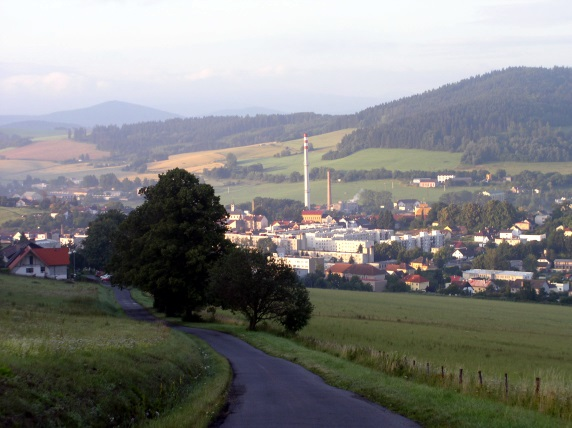
\includegraphics[scale=0.4]{kdyne.jpg}
	\end{center}
	\vspace{-10pt}
	\caption{Kdyni vévodící komín}
	\vspace{-20pt}
\end{wrapfigure}
Obec Brnířov přímo sousedí s městem Kdyně. Toto město bylo významným centrem mnoha manufaktur a dodnes zde sídlí relativně velké fabriky, které se mohou negativně podepisovat na životní prostředí města jako takového, ale i jeho okolí. To je dáno umístěním města v údolí, jemuž dominuje vysoký komín místní teplárny. Ve Kdyni je celá řada významných firem,  které se svým způsobem negativně podepisují na životním prostředí.

\subsection{Významní znečišťovatelé ve Kdyni}
Není možné zde zapsat všechny znečišťovatele, uvadím protopodle mě ty nejvýznamější: 
\begin{description}
	\item[ELITEX Machinery s.r.o.] \hfill \\
	Středně velký podnik strojírenského zaměření. Výroba strojů a linek pro výrobu papírového kartonu a krabic, výroba obráběcích stanic pro dřevozpracující průmysl, výroba extrudovacích strojů, stojanů pro přesné obráběcí stroje, textil a mnohé další.
	\item[APM Automotive s.r.o.] \hfill \\
	Široký sortiment autodílů a autopříslušenství včetně technických kapalin.
	\item[Kdynium a.s.] \hfill \\
	Slévárna vytvářející odlitky metodou voskového vytavitelného modelu. Chemické čistění a obrábění odlitků.
	\item[HAAS Bohemia s.r.o.] \hfill \\
	Drobné díly z polyurethanu a thermoplastu pro automobilový průmysl.
	\item[Teplárny Kdyně] \hfill \\
	Teplárna zajišťující ohřev vody pro většinu Kdyně spalováním uhlí.
	\item[Vodovody a kanalizace města Kdyně s.r.o.]
\end{description}

\section{Znečišťovatelé ve vzdálenějším okolí}
\begin{wrapfigure}{r}{0.4\textwidth}
	\vspace{-20pt}
	\begin{center}
		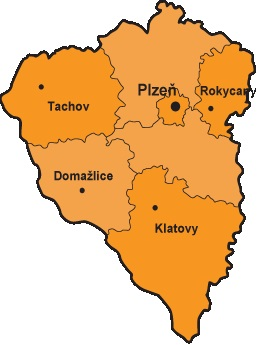
\includegraphics[scale=0.7]{plzensky_kraj.jpg}
	\end{center}
	\vspace{-10pt}
	\caption{Plzeňský kraj}
	\vspace{-20pt}
\end{wrapfigure}
Obec Brnířov i město Kdyně se nacházejí v Plzeňském kraji. Ten leží v západních Čechách. Příroda Plzeňského kraje je velmi rozmanitá a pestrá. Od horských oblastí Šumavy a Českého lesa na západní hranici s Bavorskem přes vrchovinu šumavského podhůří až ke zvlněnému vnitrozemí, všude lze nalézt kulturní krajinu s malebnými městečky a vesnicemi, lesy a vodních ploch. Pro kraj jsou typická hluboko zaříznutá údolí řek: na Šumavě Úhlavy, ve vnitrozemí zejména kaňony Střely u Rabštejna a Berounky pod Plzní.

\subsection{Voda}
% http://www.plzensky-kraj.cz/cs/kategorie/zivotni-prostredi
%\begin{center}
%	\begin{tabular}{ | l | l | l | p{7cm} |}
%	\hline
%	Day & Min Temp & Max Temp & Summary \\ \hline
%	Monday & 11C & 22C & A clear day with lots of sunshine.  
%	However, the strong breeze will bring down the temperatures. \\ \hline
%	Tuesday & 9C & 19C & Cloudy with rain, across many northern regions. Clear spells
%	across most of Scotland and Northern Ireland,
%	but rain reaching the far northwest. \\ \hline
%	Wednesday & 10C & 21C & Rain will still linger for the morning.
%	Conditions will improve by early afternoon and continue
%	throughout the evening. \\
%	\hline
%	\end{tabular}
%\end{center}
\subsection{Odpady}
\subsection{Ovzduší}
\subsection{Zemědělství}
\subsection{Lesy}

\section{Návrh na opatření ke zlepšení živ. prostředí}

\end{document}
